\subsection{Graph Layout}\label{subsec:graphlayout}

% Motivation for implementing algorithm ourselves
%   - alternative: use DOT language for Graphviz. 
%       - too much bloat and better understanding of algorithm if implemented manually
% Sugiyama framework
%   - 4 steps
%       - make graph acyclic
%           - mention trivial solution?
%       - assign states to layers
%       - order states in layers
%       - assign positions


% (CDE|(BC)+)|A works well in step 1 and 3, but it does not change from 2 to 3. I can use the reverse tregex in step 2: A|((BC)+|CDE)

% automaton is also missing dummy states

As mentioned in \cref{sec:related work}, one layout algorithm that may be used to organize and arrange the states in Timed Automata (TAs), is called the Sugiyama framework, also known as layered graph drawing \cite{Sugiyama1981}. The method comprises four steps that, when combined, results in a layered graph with minimized transition crossings. Instead of following every step of the algorithm, we are here describing a simpler version of it. The intention being to skip computation, while still obtaining a result that is ``good enough''.

\vspace{.5\baselineskip plus 2pt}
These steps are discussed below, using the TA shown on \cref{fig:graph_step0} as an example, which was constructed using the following Timed Regular Expression(TRE): $$``(CDE\mid(BC)+)\mid A"$$

% Visualise steps with different automata
\begin{center}
    \usetikzlibrary {automata,positioning}
\scalebox{0.9}{
    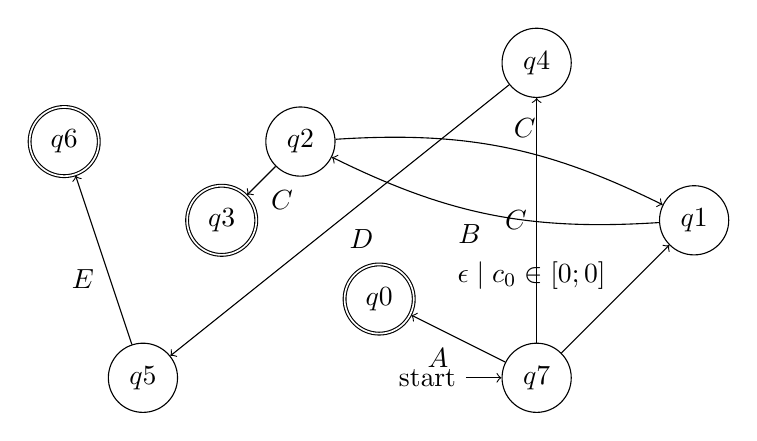
\begin{tikzpicture}[auto]
        \node[state, accepting] at (4, 1)(q0){$q0$};
        \node[state] at (8, 2)(q1){$q1$};
        \node[state] at (3, 3)(q2){$q2$};
        \node[state, accepting] at (2, 2)(q3){$q3$};
        \node[state] at (6, 4)(q4){$q4$};
        \node[state] at (1, 0)(q5){$q5$};
        \node[state, accepting] at (0, 3)(q6){$q6$};
        \node[state, initial] at (6, 0)(q7){$q7$};

        \path[->]
        (q2)edge node{$C$}(q3)
        (q1)edge [bend left=15] node{$B$}(q2)
        (q2)edge [bend left=15] node{$C$}(q1)
        (q5)edge node{$E$}(q6)
        (q4)edge node{$D$}(q5)
        (q7)edge node{$A$}(q0)
        (q7)edge node{$\epsilon\mid c_0\in[0;0]$}(q1)
        (q7)edge node{$C$}(q4)
        ;
    \end{tikzpicture}
}
\end{center}

\subsubsection{Make automata acyclic}
The first step of the Sugiyama framework is to, temporarily, make the TA acyclic. This is necessary because subsequent steps require transitions to have a consistent direction. As described by Mazetti et al., this is done by reversing a specific list of transitions \cite{Mazetti2012}.

\vspace{.5\baselineskip plus 2pt}
Since we are creating the TA, we can use the generation rules to find transitions that need to be reversed.
These reversible transitions are introduced during the iterator and absorbed iterator transformations.
Instead of reversing transitions, it is possible to omit them completely while generating the graph. This will make the algorithm simpler, since it is no longer necessary to revert the transitions back to their original orientation at the last step. However, this comes at the cost of possible transition crossings later, since the reversible transitions are no longer considered when minimizing these. A reversible transition can be seen on \cref{fig:graph_step1} (dashed line), described as $q2\rightarrow q1$.
% mention self loops

% insert image of step
\begin{center}
    \usetikzlibrary {automata,positioning}
\scalebox{0.9}{
    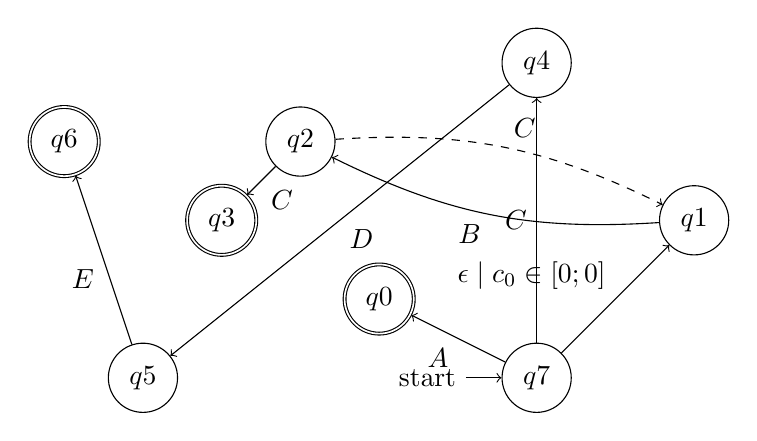
\begin{tikzpicture}[auto]
        \node[state, accepting] at (4, 1)(q0){$q0$};
        \node[state] at (8, 2)(q1){$q1$};
        \node[state] at (3, 3)(q2){$q2$};
        \node[state, accepting] at (2, 2)(q3){$q3$};
        \node[state] at (6, 4)(q4){$q4$};
        \node[state] at (1, 0)(q5){$q5$};
        \node[state, accepting] at (0, 3)(q6){$q6$};
        \node[state, initial] at (6, 0)(q7){$q7$};

        \path[->]
        (q2)edge node{$C$}(q3)
        (q1)edge [bend left=15] node{$B$}(q2)
        (q2)edge [dashed, bend left=15] node{$C$}(q1)
        (q5)edge node{$E$}(q6)
        (q4)edge node{$D$}(q5)
        (q7)edge node{$A$}(q0)
        (q7)edge node{$\epsilon\mid c_0\in[0;0]$}(q1)
        (q7)edge node{$C$}(q4)
        ;
    \end{tikzpicture}
}
\captionof{figure}{Reversible edges omitted (dashed line).}
\label{fig:graph_step1}

\end{center}

\subsubsection{Assign states to layers}
The next step is to assign states to layers. Mazetti et al. describes this process by assigning a given state to the layer index equal to the length of the longest path from the initial state. If a transition spans multiple layers, dummy states are placed to ensure that transitions only move between adjacent layers. For this step there is no simplification, as it is already simple enough for our needs. \cite{Mazetti2012}

\vspace{.5\baselineskip plus 2pt}
The result of this step can be seen on \cref{fig:graph_step2}, which has resulted in a much more structured TA.

% insert image of step
\begin{center}
    \usetikzlibrary {automata,positioning}
\scalebox{0.9}{
    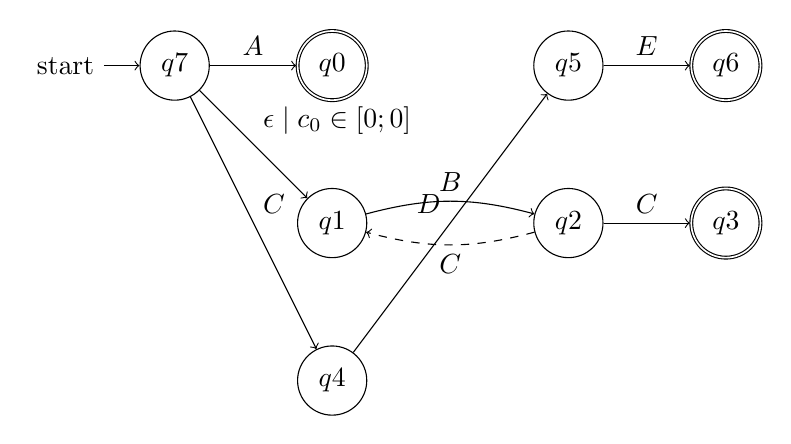
\begin{tikzpicture}[auto]
        \node[state, accepting] at (2, 0)(q0){$q0$};
        \node[state] at (2, -2)(q1){$q1$};
        \node[state] at (5, -2)(q2){$q2$};
        \node[state, accepting] at (7, -2)(q3){$q3$};
        \node[state] at (2, -4)(q4){$q4$};
        \node[state] at (5, 0)(q5){$q5$};
        \node[state, accepting] at (7, 0)(q6){$q6$};
        \node[state, initial] at (0, 0)(q7){$q7$};

        \path[->]
        (q2)edge node{$C$}(q3)
        (q1)edge [bend left=15] node{$B$}(q2)
        (q2)edge [dashed, bend left=15] node{$C$}(q1)
        (q5)edge node{$E$}(q6)
        (q4)edge node{$D$}(q5)
        (q7)edge node{$A$}(q0)
        (q7)edge node{$\epsilon\mid c_0\in[0;0]$}(q1)
        (q7)edge node{$C$}(q4)
        ;
    \end{tikzpicture}
}
\captionof{figure}{States assigned to layers.}
\label{fig:graph_step2}
\end{center}

\subsubsection{Order states in layers}
After the states have been assigned to a layer, they need to be ordered within said layer.
Mazetti et al. formulates this by sweeping through each layer and ordering its states by the barycenter (average) of the positions of its connected states in the previous layer.
E.g. if a state is connected to two states in the previous layer, and their positions are (0, 0) and (0, 100), the given state's position would be (100, 50).
This sweep is performed thrice, once forward, once backwards, and lastly, forward again.
This ensures that both a given state's incoming and outgoing states play a role in minimizing transition crossings. \cite{Mazetti2012}

\vspace{.5\baselineskip plus 2pt}
The algorithm described above, is applied to the example, and the result can be seen on \cref{fig:graph_step3}.
% insert image of step
\begin{center}
    \usetikzlibrary {automata,positioning}
\scalebox{0.9}{
    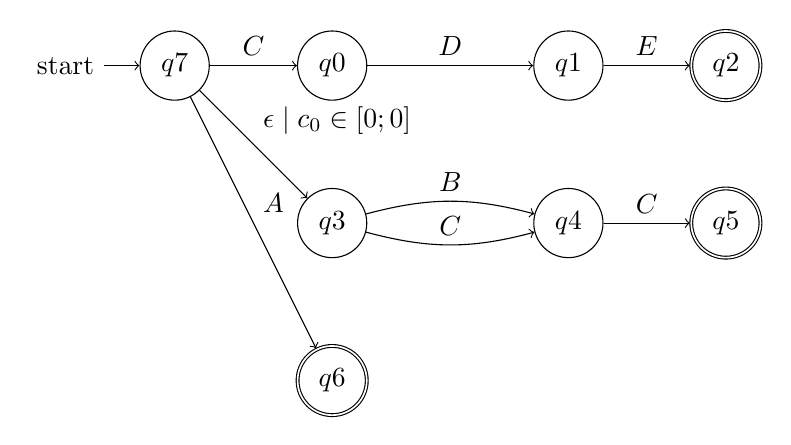
\begin{tikzpicture}[auto]
        \node[state] at (2, 0)(q0){$q0$};
        \node[state] at (5, 0)(q1){$q1$};
        \node[state, accepting] at (7, 0)(q2){$q2$};
        \node[state] at (2, -2)(q3){$q3$};
        \node[state] at (5, -2)(q4){$q4$};
        \node[state, accepting] at (7, -2)(q5){$q5$};
        \node[state, accepting] at (2, -4)(q6){$q6$};
        \node[state, initial] at (0, 0)(q7){$q7$};

        \path[->]
        (q1)edge node{$E$}(q2)
        (q0)edge node{$D$}(q1)
        (q4)edge node{$C$}(q5)
        (q3)edge [bend left=15] node{$B$}(q4)
        (q3)edge [bend right=15] node{$C$}(q4)
        (q7)edge node{$C$}(q0)
        (q7)edge node{$\epsilon\mid c_0\in[0;0]$}(q3)
        (q7)edge node{$A$}(q6)
        ;
    \end{tikzpicture}
}


\end{center}

\subsubsection{Assign positions}
The last step is to assign positions to each state.
Since the last few steps already significantly improve visual clarity, the approach described by Mazetti et al., has been omitted in favor of a simpler algorithm. Instead, states are placed based on their layer, and their index on said layer, which already offers much visual clarity. It should also be noted, that reversible transitions are reintroduced at this step too. This is reflected in the TA on \cref{fig:graph_step4}.

% insert image of step
\begin{center}
    \usetikzlibrary {automata,positioning}
\scalebox{0.9}{
    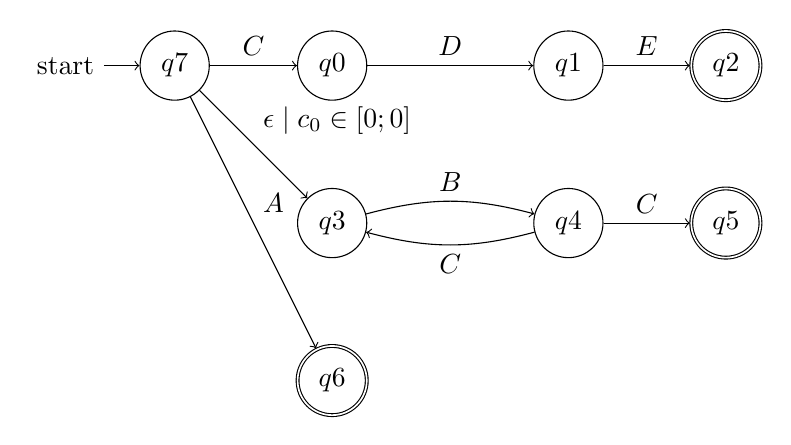
\begin{tikzpicture}[auto]
        \node[state] at (2, 0)(q0){$q0$};
        \node[state] at (5, 0)(q1){$q1$};
        \node[state, accepting] at (7, 0)(q2){$q2$};
        \node[state] at (2, -2)(q3){$q3$};
        \node[state] at (5, -2)(q4){$q4$};
        \node[state, accepting] at (7, -2)(q5){$q5$};
        \node[state, accepting] at (2, -4)(q6){$q6$};
        \node[state, initial] at (0, 0)(q7){$q7$};

        \path[->]
        (q1)edge node{$E$}(q2)
        (q0)edge node{$D$}(q1)
        (q4)edge node{$C$}(q5)
        (q3)edge [bend left=15] node{$B$}(q4)
        (q4)edge [bend left=15] node{$C$}(q3)
        (q7)edge node{$C$}(q0)
        (q7)edge node{$\epsilon\mid c_0\in[0;0]$}(q3)
        (q7)edge node{$A$}(q6)
        ;
    \end{tikzpicture}
}


\end{center}
